\documentclass[12pt, letterpaper]{article}
\usepackage{setspace}
\usepackage{subcaption}
\usepackage[font={small,it}]{caption}\usepackage{graphicx}
\usepackage{array}
\usepackage{longtable}
\usepackage{quotes}
\usepackage{amsmath}
\usepackage{hyperref}
\usepackage[skip=10pt plus1pt, indent=40pt]{parskip}

% set reference files
\usepackage{biblatex}
\addbibresource{references.bib}

% set margins
\usepackage{geometry}
\geometry{margin=1in}

% Remove paragraph indentation
\setlength{\parindent}{0pt}


\graphicspath{{./figs/}{c:/Users/Zayan/Documents/code/personal_repos/neural_nets/ECE_8770/project_2/results}}
\onehalfspacing

\begin{document}

\begin{titlepage}
    \begin{center}

        \vspace*{1cm}

        \Large
        \textbf{ECE 8870 Project 2}

        \vspace{0.5cm}
        \textbf{Qazi Zarif Ul Islam}

        Pawprint: qzic2d

        \large

        \vspace{0.8cm}
        % \includegraphics[width=0.4\textwidth]{figs/Screenshot 2023-09-28 011032.png}

        University of Missouri-columbia \\
        04/21/2024
        
    \end{center}
\end{titlepage}

\section{Technical Description}

In this project, an RNN and an LSTM were implemented using pytorch.
The broader goal of this project was to understand the working principles of
RNNs and LSTMs and gain a comparative understanding of the two neural network
architectures. 

In the following sections, first the basic components of an RNN and an LSTM 
are introduced as well as an explanation of how backpropagation occurs in an 
RNN. This explanation will be more qualitative than mathematically rigorous. 
A more extensive treatment of backpropagation in RNNs can be found in ---. After that, the experiments and results shall be demonstrated and discussed before
a final conclustion section that talks about what more can be done to understand
RNNs and LSTMs and the deficiencies of this project.

\subsection{Recurrent Neural Networks}

Recurrent Neural Networks are neural neural networks that store the 
hidden layer's output at the current time step so that it can influence
the output of the hidden layer at the next time step. Qualitatively,
this is commonly thought of as information being passed to the next time
step. 

\begin{figure}[htpb]
    \centering
    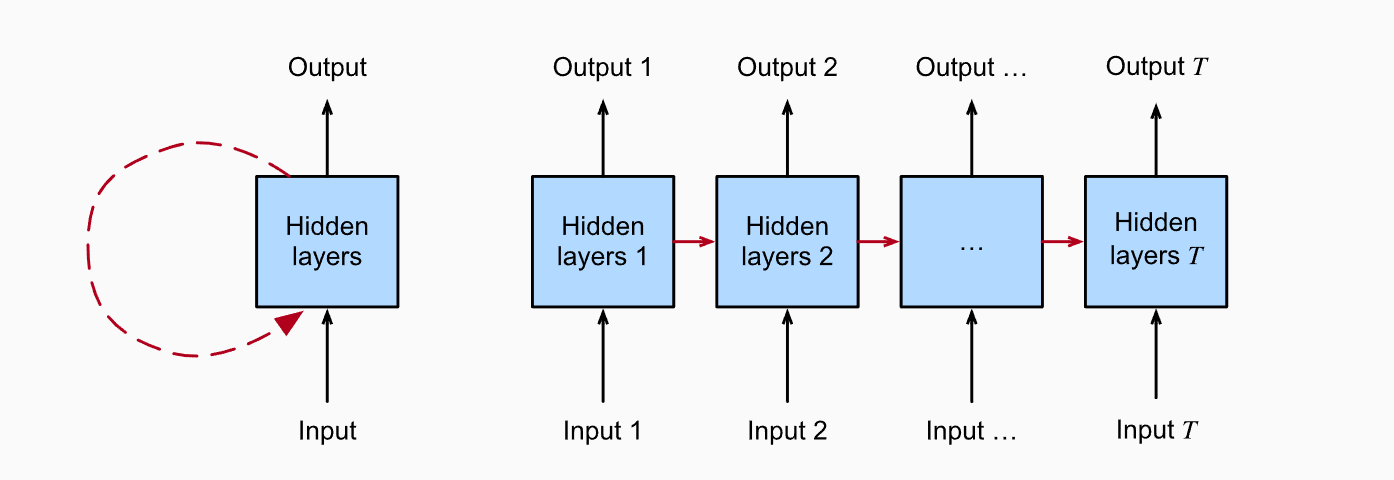
\includegraphics[width=0.8\textwidth]{d2l_ai_rnn_v1.png}
    \caption{Fig 1: On the left recurrent connections are depicted via cyclic edges. 
    On the right, we unfold the RNN over time steps. Here, recurrent edges span 
    adjacent time steps, while conventional connections are computed synchronously}
\end{figure}

\printbibliography

\end{document}